 \begin{frame}{reprogramming}{introduction}
    \begin{itemize}
        \item   \textbf{observation}
            \begin{itemize}
                \item   pre-trained deep models can be very powerful if trained with sufficient data, even for different tasks
            \end{itemize}
        \bigskip
        \item   \textbf{idea}
            \begin{itemize}
                \item re-using pre-trained models for a new task \textbf{without} re-training
            \end{itemize}
        \bigskip
        \item<2->   \textbf{goals}
            \begin{itemize}
                \item   keep number of training parameters minimal
                \item   utilize unmodified network trained on different task
            \end{itemize}
    \end{itemize}
\end{frame}

\begin{frame}{reprogramming}{overview}
    \begin{itemize}
        \item   inspired by
            \begin{itemize}
                \item   transfer learning
                \item   adversarial learning
            \end{itemize}
        \item   allows for small trainable model (input and output processing)
    \end{itemize}
    \vspace{-2mm}
    \begin{figure}%
        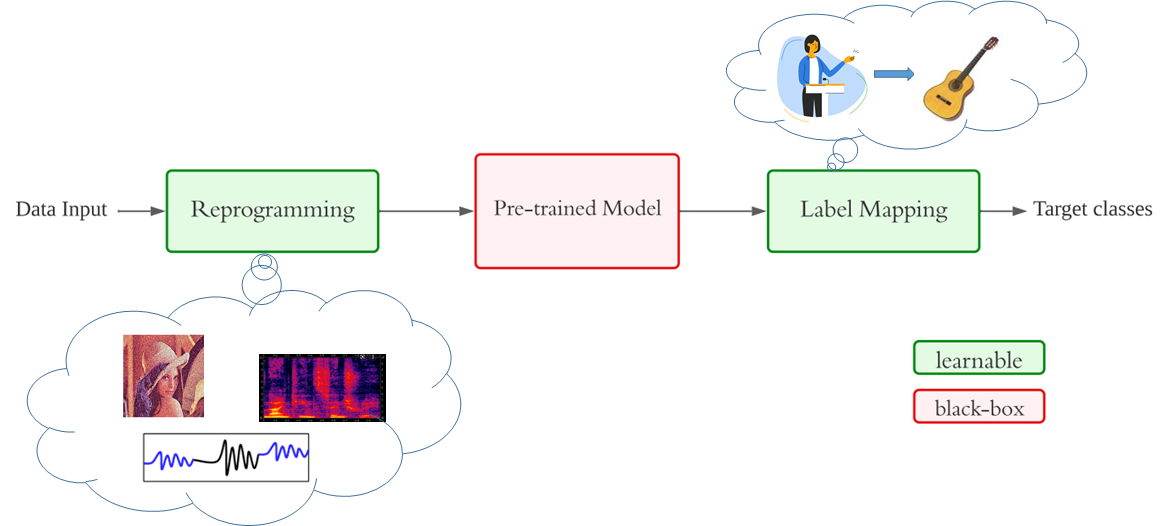
\includegraphics[width=.8\linewidth]{reprogramming}%
    \end{figure}
\end{frame}

\begin{frame}{reprogramming}{experimental setup: data}
    \begin{columns}
        \column{.8\linewidth}
            \begin{itemize}
                \item   OpenMic:
                    \begin{itemize}
                        \item   20 classes of musical instruments
                        \item   \unit[10]{s} audio snippets (20000)
                    \end{itemize}
            \end{itemize}
        \column{.2\linewidth}
    \end{columns}
\end{frame}

\begin{frame}{reprogramming}{experimental setup: baselines}
    \begin{itemize}
        \item Baseline AST:
            \begin{itemize}
                \item   state of the art performance on audio event classification\footfullcite{gong_ast_2021}
            \end{itemize}
        \bigskip
        \item   ablation study:
            \begin{itemize}
                \item   CNN only
                \item   U-Net only
                \item   CNN + AST + FC
                \item   U-Net + AST + FC
            \end{itemize}
    \end{itemize}
\end{frame}

\begin{frame}{reprogramming}{results: classification metrics}
    \begin{columns}
    \column{.7\linewidth}    
    \begin{footnotesize}
    \begin{table}[]
        \centering
        \begin{tabular}{l | c | c c c c c c c c c}
           method & F1 (macro) & train. param. (M) \\
           \hline
            AST + simple output mapping & 62.03 & 0.001\\
            CNN & 60.77 & 0.017\\
            U-Net & 62.73 & 0.017\\
            CNN + AST + FC & 78.08 & 0.017\\
            U-Net + AST + FC & \textbf{81.60} & 0.018
           
        \end{tabular}
    \end{table}
    \end{footnotesize}
    \column{.3\linewidth}
    \begin{figure}%
    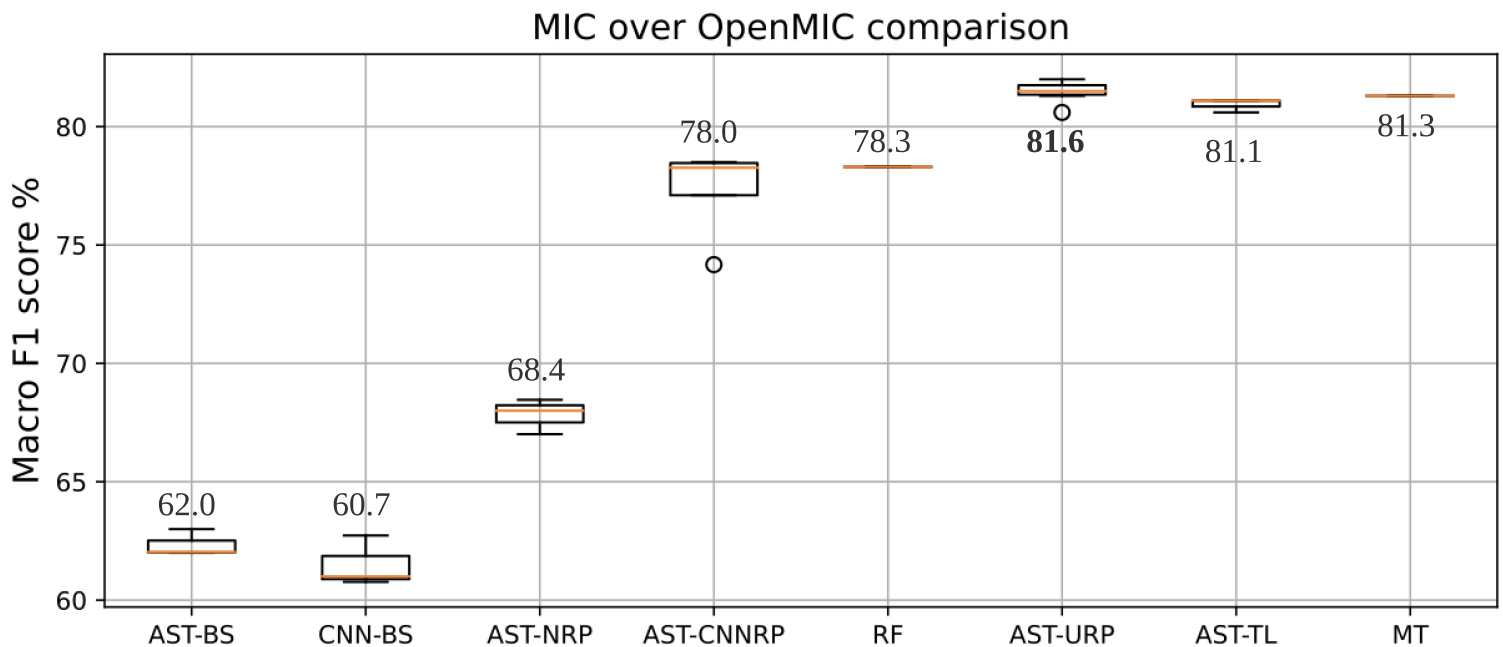
\includegraphics[width=\columnwidth]{reprog-results}%
    \end{figure}
    \end{columns}
    
    \begin{itemize}
        \item   a powerful model trained on a different task cannot easily be used directly
        \item   proper input and output processing can significantly improve performance
        \item   \textit{re-programming can beat the state-of-the-art} with a fraction of trainable parameters (at least factor 10)
    \end{itemize}
    \phantom{\footfullcite{chen_music_2023}}
\end{frame}

